\documentclass[oneside]{article}
\usepackage[T1]{fontenc}
\usepackage[utf8]{inputenc}
\usepackage{alphabeta}
\usepackage[margin=0.9in]{geometry}
\usepackage{amsmath,amssymb}
\usepackage{graphicx}


\title{ASE summaries 18-19}
\date{\today}

\date{\today}
\begin{document}

\maketitle

\section{XML (XML - Extensible Markup Language)}
\begin{itemize}
    \item XML is a language used for the description and delivery of marked up electronic text over the Web. It comprehends the concept of \textit{document type} and the concept of \textit{portability over different computing environments}. An XML document is composed of named \textit{containers} and their contained data values;
    
    \item since XML allows designers to choose their own names, it provides a mechanism of \textbf{namespaces} as a way of distinguishing between elements that use the same local name but are actually different. It is possible to use global namespace for the document or to assign locally a namespace to a placeholder;
    
    \item a way for defining XML tags and structure is with \textbf{schemas}: documents that clearly define the content of, and structure of, and a class of XML documents. The \textbf{XML Schema Definition Language (XSD)}, provides a type system for XML processing environments;
    
    \item a construct that declares elements may use \textbf{compositors} to aggregate existing types into a structure. Compositors are: \textit{sequence}, \textit{choice}, \textit{all}, \textit{minOccur} and \textit{maxOccur};
    
    \item complex types can be either \textbf{extended} or \textbf{restricted} to implement the inerithance;
    
    \item schemas can be \textbf{imported} or \textbf{included} into other ones;
\end{itemize}


% ========================================
% ========================================


% ========================================
% ========================================


\section{REST (REST - REpresentational State Transfer)}
\begin{itemize}
    \item it was originally proposed as an architectural style as a lighter alternative to SOAP for message exchange;
    
    \item it was developed as an abstract model of the Web architecture, needed to guide the redesign and definition of HyperText Transfer Protocol (HTTP) and Uniform Resource Identifiers (URI);
    
    \item in contrast with the complexity of WS* standards, RESTful services constitute a simpler approach to build service-oriented architectures.
    
    \item REST principles are the following.
    \begin{itemize}
        \item resources are exposed by a RESTful service and identified by \textbf{URIs}, which provide a global addressing space for resource and service discovery; 
        \item resources are manipulated using HTTP methods (\textit{PUT}, \textit{GET}, \textit{POST} and \textit{DELETE}); 
        \item the RESTful approach is \textbf{message-centric}, since all services operate on data by means of request/response mechanism. Furthermore, resources are decoupled from their representation so that their content can be accessed in various formats;
    \end{itemize}
    
    \item \textbf{PROS}: simplicity and very low learning curve, scalability, efficiency and deployment simplicity;
    \item \textbf{CONS}: complex interfaces and resources are not easy to be represented as URLs, no prescriptive best practices, management and monitoring of \textit{QoS} must be implemented by hand, easy decisions may lead to significant development waiding and technical risks;
    
    \item REST is for simple and running in short time span applications, while WS-* is preferable for professional and enterprise applications;
\end{itemize}


% ========================================
% ========================================


% ========================================
% ========================================


\section{SOAP (SOAP - Simple Object Access Protocol)}
\begin{itemize}
    \item it is an XML based standard tat relies on HTTP as transport protocol to enable the communication among separate systems running on heterogeneous infrastructures;
    
    \item it is a stateless, one-way network application protocol that is used to transfer messages between service instances described by WSDL interfaces;
    
    \item SOAP messages are carried as HTTP requests and responses where endpoints are HTTP based URLs
    
    \item each message consist of an \textbf{envelope} containing an optional \textbf{header}, which contains information relevant how to the message must be processed (e.g. where the document must be sent, where it originated and signatures informations), and a mandatory \textbf{body}, which contains an application specific payload (data, parameters to a method call) or a fault message, but not both;
    
    \item SOAP supports two possible communication styles: the \textbf{RPC}, where web services appears as a remote object to a client application, or the \textbf{document style};
    
    \item \textbf{PROS}: simple, portable, firewall-friendly, interoperative and open;
    
    \item \textbf{CONS}: bound to HTTP and stateless;
\end{itemize}


% ========================================
% ========================================


% ========================================
% ========================================


\section{WSDL (WSDL - Web Service Description Language)}
\begin{itemize}
    \item WSDL is an XML based language that provides a model to describe SOA based application. It describes web services in a consistent manner so that they can be published by service providers, and discovered and invoked by clients and developers;
    
    \item by providing the means to group messages into operations and operations into interfaces, it is used to describe: \textit{what a service S does} (operations), \textit{where it resides} (URI) and \textit{how to invoke it} (transport protocol and parameters);

    \item a \textbf{WSDL interface} represents a service contract between the service requester and the service provider, in much the same way object oriented programming interfaces work. It is platform independent and primarily used to describe SOAP enabled services;
    
    \item a WSDL description consist of two distinct parts: an \textbf{abstract service description} with the operations supported by the service, their parameters and abstract data types, and a \textbf{concrete endpoint implementation} which binds the abstract interface to an actual network address, to a specific protocol and to a concrete data structures;
    
    \item a service can support many bindings to the same abstract interface, accessible to a distinct endpoints;
    
    \item to realize above functions, the WSDL document is dived into five parts: \textbf{types} (defines the (XML Schema) data types used by the web service), \textbf{message} (defines the data elements for each operation), \textbf{port type} (describes the operations that can be performed and the messages involved), \textbf{binding} (defines the protocol and data format for each port type) and \textbf{service} (defines the supported protocols by the web service);
\end{itemize}

\begin{figure}[!htb]
    {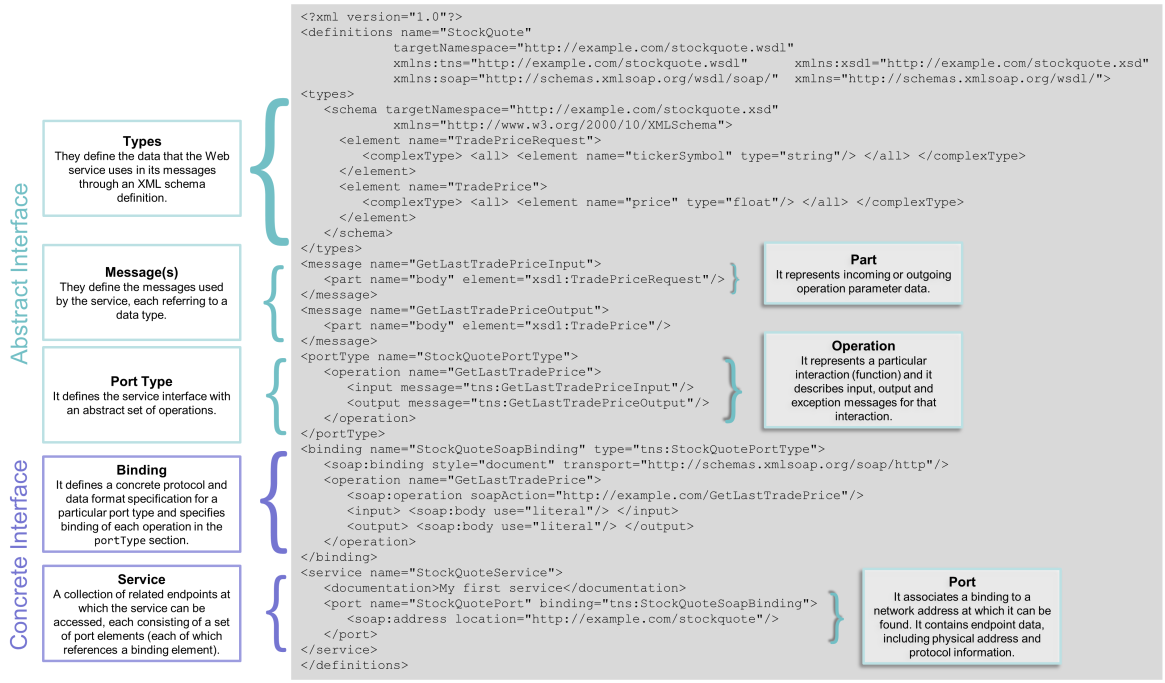
\includegraphics[width=\textwidth]
    {WSDL_elements.png}}
\end{figure}


% ========================================
% ========================================


% ========================================
% ========================================

\newpage
\section{BPM - BPMN}
\begin{itemize}
    \begin{figure}[!htb]
        \makebox[\textwidth][c]{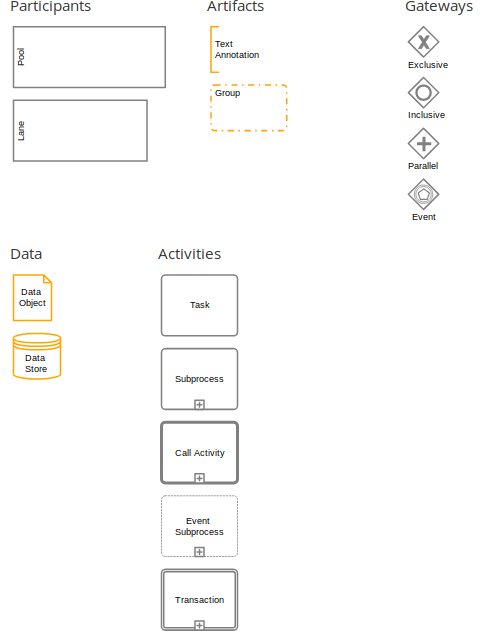
\includegraphics[width=0.50\textwidth]{bpmn_elements.png}}
    \end{figure}
    \item a \textbf{business process} consists of a set of activities that are performed in coordination in an organizational and technical environment. These activities jointly realize a business goal. Each business process is enacted by a single organization, but it may interact with business processes performed by other organizations;
    
    \item a \textbf{business process model} consists of a set of activity models and execution constraints among them. A \textbf{business process instance} represents a concrete case in the operational business of a company, consisting of activity instances;
    
    \item the \textbf{Business Process Model and Notation (BPMN)} is a graphical representation for specifying business processes in a business process model;
    
    \item in BPMN \textbf{gateways} control token flow in a process. They allow modelling decisions based on data and events as well as fork/join concurrency. Types are:
        \begin{itemize}
            \item \textbf{parallel gateway}: it is used to forking into multiple paths of execution or joining multiple incoming paths of execution. In \textbf{fork processes},  all outgoing sequence flows are followed in parallel, creating one concurrent execution for each sequence flow. In \textbf{join processes} all concurrent executions arriving at the parallel gateway wait at the gateway until an execution has arrived for each of the incoming sequence flows. Then the process continues past the joining gateway. An important difference with other gateway types is that the parallel gateway does not evaluate conditions;
            \item \textbf{exclusive gateway (XOR)}: it is used to model a decision in the process. When the execution arrives at this gateway, all outgoing sequence flows are evaluated in the order in which they have been defined. The sequence flow which condition evaluates to ‘true’ (or which doesn't have a condition set, conceptually having a ‘true’ value defined on the sequence flow) is selected for continuing the process. Note that only one sequence flow is selected when using the exclusive gateway. In case of multiple sequence flow are true, the first one is selected. If no sequence flow can be selected this will result in a runtime exception, unless you have a default flow defined;
            \item \textbf{inclusive gateway}: it can be seen as a combination of an exclusive and a parallel gateway. Like an exclusive gateway, you can define conditions on outgoing sequence flows and the inclusive gateway will evaluate them. However, the main difference is that the inclusive gateway can receive more than one sequence flow, like a parallel gateway. In \textbf{fork processes}, all outgoing sequence flow conditions are evaluated and for the sequence flow conditions that evaluate to ‘true’, the flows are followed in parallel, creating one concurrent execution for each sequence flow. For \textbf{join processes}, all concurrent executions arriving at the inclusive gateway wait at the gateway until an execution has arrived for each of the incoming sequence flows that have a process token. This is an important difference to the parallel gateway. So in other words, the inclusive gateway will only wait for the incoming sequence flows that are executed;
        \end{itemize}
        
    \item \textbf{error event}: they are events which are triggered by a defined error.
    
    \item \textbf{Camunda} is a java-based, open-source workflow and decision automation platform. It ships with tools for creating workflow and decision models, operating deployed models in production, and allowing users to execute workflow tasks assigned to them. It provides a BPMN standard compliant workflow engine and a DMN standard compliant decision engine, which can be embedded in Java applications and with other languages via REST. Typical use cases for the Camunda can be microservices orchestration and human task management;
    
    \item \textbf{(service) orchestration} represents a single centralized executable business process (the \textit{orchestrator}) that coordinates the interaction among different services. The \textit{orchestrator} is responsible for invoking and combining the services. \newline
    \textbf{service choreography} is a global description of the participating services, which is defined by exchange of messages, rules of interaction and agreements between two or more endpoints. \textit{Choreography} employs a decentralized approach for service composition. \newline
    The choreography describes the interactions between multiple services, where as orchestration represents control from one party's perspective. This means that a choreography differs from an orchestration with respect to where the logic that controls the interactions between the services involved should reside;
    
    \item \textbf{from gateways to workflow nets}: see attachment
\end{itemize}


% ========================================
% ========================================


\section{Petri Nets}
\begin{itemize}
    \item \textbf{Petri nets} are directed bipartite graph with two nodes types, \textbf{places} and \textbf{transitions}. Nodes are connected via directed arcs and connections between two nodes of the same type are not allowed. A Petri net is a triple \textbf{(P, T, F)} where P is a finite set of places, T is a finite set of transition and $F \subseteq (P \times T) \cup (T \times P)$ is a finite set of arcs (flow relation)
    
    \item a place \textit{p} is called an \textbf{input place} of a transition \textit{t} $\in$ \textit{T} if and only if there exists a directed arc from \textit{p} to \textit{t}. A place \textit{p} is called an \textbf{output place} of a transition \textit{t} $\in$ \textit{T} if and only if there exists a directed arc from \textit{t} to \textit{p};
    
    \item at any time a place can contain zero or more \textbf{tokens};
    
    \item a \textbf{state M}, also referred to as \textit{marking}, of a Petri net is a distribution of tokens over the places;
    
    \item a transition \textit{t} is \textbf{enabled} if and only if each input place \textit{p} of \textit{t} contains at least one token;
    
    \item an enabled transition may \textbf{fire}: if transition \textit{t} fires, then \textit{t} consumes one token from each input place \textit{p} of \textit{t} and produces one token in each output place \textit{p} of \textit{t};
    
    \item a state $M_n$ is \textbf{reachable} from a state $M_1$ if and only if there is a firing sequence $t_1$, $t_2$, ..., $t_{n-1}$ such that $\mathcal{$M_1$}\overset{t_1}{\longrightarrow}\mathcal{$M_2$}\overset{t_2}{\longrightarrow}$ ... $\overset{t_{n-1}}{\longrightarrow}\mathcal{$M_n$}$;

\end{itemize} \begin{itemize}

    \item a Petri net (PN, M) is \textbf{live} if and only if for every reachable state $M'$ and every transition \textit{t}, there is a state $M''$ reachable from $M'$ which enables \textit{t};
    
    \item a Petri net (PN, M) is \textbf{bounded} if and only if for each place \textit{p} there is a $n \in N$ such that for every reachable state the number of tokens in \textit{p} is less than \textit{n};
\end{itemize}


% ========================================
% ========================================


% ========================================
% ========================================


% ========================================
% ========================================


\section{Workflow Nets}
\begin{itemize}
    \item a Petri net is a \textbf{workflow net} if and only if there is a source place with no incoming edges and there is a sink place with no outcoming edge, and all places and transition are located on some path from the source place to the sink place;
    
    \item more specifically, a Petri net \textit{PN = (P,T,F)} is a \textit{workflow net} if and only if:
        \begin{itemize}
            \item \textit{PN} has a special place source $i \in P$ with non incoming edge and a special sink place $o \in P$ with no outcoming edge;
            \item if we add a transition $\bar t$ which connect place \textit{o} with \textit{i} then the resulting Petri net is strongly connected;
        \end{itemize}
    
    \item a workflow is \textbf{sound} if and only if:
        \begin{itemize}
            \item every execution starting from the initial marking eventually leads to the final marking:
            \item every transition occurs in at least one net execution
        \end{itemize}

    \item workflow net transitions can be annotated with triggers, to denote who or what is responsible for an enabled transition of fire;
    
    \item more specifically, a workflow net \textit{WN = (P;T;F)} is \textit{sound} if and only if:
    \begin{itemize}
        \item $\forall M (\{i\} \overset{*}\longrightarrow M) \Longrightarrow (M \overset{*}\longrightarrow \{o\})$
        \item $\forall M (\{i\} \overset{*}\longrightarrow M \land M \geq \{o\}) \Longrightarrow (M = \{0\})$
        \item $\forall t \in T \exists M, M' | \{i\} \overset{*}\longrightarrow M \overset{t}\longrightarrow M'$
    \end{itemize}
    
    \item consider also the following \textbf{theorem}: a workflow net N is \textit{sound} if and only if $(\tilde N,i)$ is live and bounded, where $\tilde N$ is N extended with a transition from the sink place \textit{o} to the source place \textit{i};
\end{itemize}


% ========================================
% ========================================


% ========================================
% ========================================


% ========================================
% ========================================


\section{Microservices}
\begin{itemize}
    \item the term \textbf{microservices} describes the particular way of designing applications as suites of independently deployable services;
    
    \item \textit{microservices style} is an approach developing a single application as a suite of small services, each running on its own process and communicating with lightweight mechanisms, often an HTTP resource API. These services are built around business capabilities and independently deployable by fully automated deployment machinery;
    
     \item as well as the fact that microservices are independently deployable and scalable, each service also provides a firm module boundary, even allowing for different services to be written in different programming languages;
     
     \item we can compare a \textbf{service} to a \textbf{component}, a unit of software that is independently replaceable and upgradeable. A service differs from \textbf{library} since the former is out-of-process components which communicates with a mechanism such as a web service request or a remote procedure call, and the latter are components linked to program and called using in-memory function calls;
        
    \item the microservices approach to \textbf{division of software} is to split up into services organized around \textit{business capability}. To do this, teams are \textbf{cross functional}, including the full range of skills required for the development. Moreover, cross functional teams are responsible for building and operating each product and each product is split into a number of individual services communicating via a message bus;
    
    \item in the microservices view, a team should own a product over its full lifetime, in the sense that a development team takes full responsibility for the software production (\textit{they build it, they run it}). This model brings developers into day-to-day contact with how their software behaves in production and increases contact with their users, as they have to take on at least some of the support burden;
    
    \item the microservices community favours an alternative approach about the communication between services: \textbf{smart endpoints and dumb pipes}. Applications built from microservices aim to be as decoupled and cohesive as possible, receiving a request, applying a logic and producing a response using simple "RESTish" protocols. Another approach is to message over a lightweight message bus (e.g. RabbitMQ or ZeroMQ);
    
    \item regarding \textit{services contracts}, teams building microservices, rather than use a set of defined standards written down somewhere on paper, prefer the idea of producing useful tools that other developers can use to solve similar problems to the ones they are facing. The two most used patterns are \textbf{tolerant-reader} (be as tolerant as possible when reading data from another service) and \textbf{consumer-driven contracts} (each consumer captures their expectations of the provider in a separate contract, which is shared with the provider which must fulfill for each client). These techniques and the tooling growing up around them, limit the need for central contract management by decreasing the temporal coupling between services;
    
    \item regarding the \textbf{data management}, microservices prefer to decentralize data storage using the \textbf{polyglot persistence} approach: they prefer letting each service manage its own database, either different instances of the same database technology or entirely different database systems. But decentrylizing responsibility or data across microservices has implications for managing updates: the common approach in microservices architecture to solve it is to \textbf{emphasize transactionless coordination between services}, since transactions imposes significant temporal coupling which is problematic across multiple services;
    
    \item to automate the process of deploy of microservices, teams that adopt this style make an intensive use of \textit{Continuous Integration} and \textit{Continuous Delivery}: to do that, a lot of \textbf{automated test} are done and an \textbf{automate delivery} process is adopted;
    
    \item a consequence of using microservices as component is that applications need to be designed so that they can tolerate the failure of services: since services can fail at any time, it's important to be able to detect failures quickly and, if possible, automatically restore service. It can be done with \textbf{semantic monitoring}, that is on \textit{real-time monitoring} of the application checking architectural elements or business relevant metrics. Monitoring is vital to spot bad emergent behavior quickly so it can be fixed;
    
    \item the key property of a component is the notion of independent replacement and upgradeability, which implies that we look for points where we can imagine rewriting a component without affecting its collaborators;
    
    \item it is recommended, when start to writing a new application, to shouldn't start with a microservices architecture, but begin with a monolith, keep it modular and split it into microservices once the monolith becomes a problem;
    
    \begin{figure}[!htb]
      \makebox[\textwidth][c]{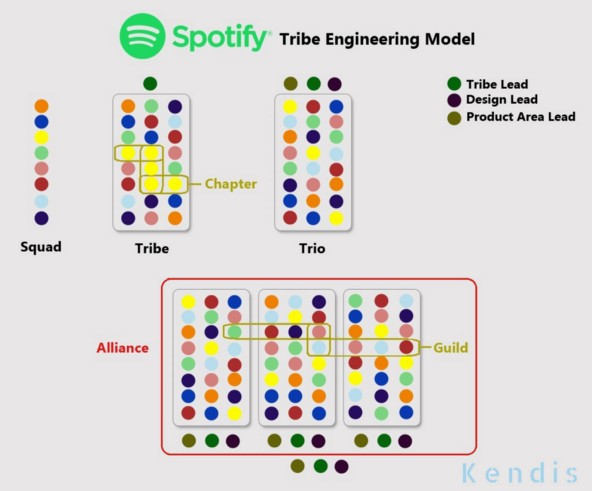
\includegraphics[width=0.6\textwidth]{spotify_schema.png}}
    \end{figure}
    
    \item the \textbf{Spotify Tribe Engineering Model} is the Spotify product development. Spotify is a 100\%-Agile company that started with the Scrum framework, but as their teams were growing, they noticed some things on the Scrum framework that weren’t working well for them. The new elements of this engineering model are:
        \begin{itemize}
            \item \textbf{Squads}: similar to scrum teams, they are small cross-functional, self-organized team usually with less than eight members. The team members have end-to-end responsibilities, and they work together towards their long-term mission.A squad is autonomous, self-organizing and self-managing. Each squad has a mission to accomplish and is free to choose an agile methodology. Each squad has direct contact with stakeholders;
            
            \item \textbf{Tribes}: they are a collection of squads within the same business area. A tribe may consist of 40–150 people but ideally, a tribe should have max. 100 individuals. A tribe has a tribe lead responsible for creating a productive and an innovative environment for the squads;
            
            \item \textbf{Chapters}: they are specialist at the horizontal level of the functional organization. A chapter consists of individuals from different squads to be grouped into one and formed within a tribe;
            
            \item \textbf{Guilds}: they are informal groups constituted of people from different tribes, who have a common interest, form a guild. A person from any squad, chapter or tribe can be a part of a guild. The purpose of having both chapters and guilds
            
            \item \textbf{Trio}: it is formed when for every tribe there is a design, product area and a tribe lead;
            
            \item \textbf{Alliance}: it is a combination of three trios. It is led by a product, design and a tribe lead;
            
            \item \textbf{Chief Architect}: it is a crucial bember of organizations who defines architectural vision, guides in designs and deals with the system architecture dependency issues;
    \end{itemize}
    
    \textbf{Benefits} of this development model are: enhanced velocity, processes are reduced to a minimum, addresses short term challenges, minimized dependencies, lack of a firm structure makes problem solving easier, minimum control, promotes clarity and transparency, works best for what suits your working environment;
    
    \item \textbf{Fault Injection Testing}: FIT is a software testing method which deliberately introduces errors to a system to ensure it can withstand and recover from error conditions. FIT is typically carried out prior to deployment to uncover any potential faults that may have been introduced during production. Similar to stress testing, fault injection testing is used to identify specific weaknesses in a hardware or software system so they can be fixed or avoided;
    
    \item \textbf{Design for Failure}: The concept of DfF is often used to describe the approach that assumes that there will be an hardware or system failure somewhere, sometime and, instead of architecting for hardware and server clustering and availability, to design applications so that recovery can be performed quickly.
    
    \item Some definition:
        \begin{itemize}
            \item \textbf{Git}/\textbf{GitHub}: it is a distributed version control system for tracking changes in source code during software development. It is designed for coordinating work among programmers, but it can be used to track changes in any set of files. Its goals include speed, data integrity, and support for distributed, non-linear workflows. Every Git directory on every computer is a full-fledged repository with complete history and full version-tracking abilities, independent of network access or a central server.
            
            \item \textbf{Flask}: it is a micro web framework written in Python. Flask does not include a database abstraction layer, form validation or anything else where different libraries already exist that can handle that. Instead, Flask supports extensions to add such functionality to your application as if it was implemented in Flask itself. Numerous extensions provide database integration, form validation, upload handling, various open authentication technologies, and more;
            
            \item \textbf{MVC pattern}: it is an architectural pattern commonly used for developing user interfaces that divides an application into three interconnected parts. The MVC design pattern decouples these major components allowing for code reuse and parallel development. Traditionally used for desktop graphical user interfaces (GUIs), this architecture has become popular for designing web applications;
            \begin{figure}[!htb]
              \makebox[\textwidth][c]{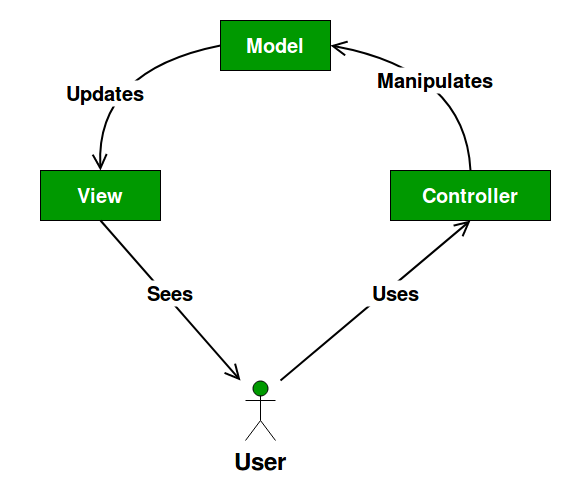
\includegraphics[width=0.35\textwidth]{mvc_pattern.png}}
            \end{figure}
            
            \item \textbf{Celery}: it is a distributed system for processing messages on a task queue with a focus or real-time processing and support for task scheduling. Celery communicates with a message broker and distributes work. The execution units, called tasks, are executed concurrently on one or more worker nodes. Tasks can execute asynchronously (in the background) or synchronously (wait until ready). Celery is used in production systems to process millions of tasks every day;
            
            \item \textbf{OpenAPI}: originally known as the Swagger Specification, it is a specification for machine-readable interface files for describing, producing, consuming, and visualizing RESTful web services. Applications implemented based on OpenAPI interface files can automatically generate documentation of methods, parameters and models. This helps keep the documentation, client libraries, and source code in sync. It is language-agnostic: with OAPI clients can understand and consume services without knowledge of server implementation or access to the server code. \newline \textit{OpenAPI = Specification, Swagger = Tools for implementing the specification};
        \end{itemize}
\end{itemize}


% ========================================
% ========================================


% ========================================
% ========================================


\section{Software Testing}
\begin{itemize}
    \item \textbf{testing process} is intended to show that a program does what is intended to do and to discover program defects before it is put into use. When we test a software, we execute a program using artificial data;
    
    \item it is different from \textbf{debugging}, which is the process of locating problems with the code and changing the program to fix these problems;
    
    \item when we test a software we are trying to:
        \begin{itemize}
            \item demonstrate to the developer and the customer that the software meets its requirements. This process is called \textbf{validation testing} and we expect the system to perform correctly using a set of test cases that reflect the system's expected use;
            \item find inputs or input sequences where the behavior of the software is incorrect, undesirable or does not conform to its specification. This process is called \textbf{defect testing} in which test cases are designed to expose defects
        \end{itemize}
    
    \item it is important to say that testing cannot demonstrate that software is free of defects or that it will behave as specified in every circumstance, in fact \textit{testing can only show the presence of errors, not their absence};
    
    \item \textbf{software verification} is the process of checking that the software meets its stated functional and non-functional requirements, while \textbf{software validation} is to ensure that the software meets the customer's expectations. In short terms, the goal if verification and validation process is to establish confidence that the software system is "fir for purpose", namely that the system must be good enough for its intended use;
    
    \item the level of required confidence depends on:
        \begin{itemize}
            \item \textbf{software purpose}: the more critical the software, the more important it is that it is reliable;
            \item \textbf{user expectations}: because their previous experience with buggy, unreliable software, users have low expectations of software quality at the beginning. But when that software product becomes more established, users expect it to become more reliable;
            \item \textbf{marketing environment}: when a software company brings a system to market, it must take into account competing products, the price that customers willing to pay for a system and the required schedule for delivering that system. If a software product or app is very cheap, users may be willing tolerate a lower level of reliability;
        \end{itemize}
        
    \item V\&V process may involve also software \textbf{inspections} and \textbf{reviews}. These are static techniques in which software isn't executed. Inspections mostly focus on the source code of the system, but any readable representation of the software, such as its requirements or a design model, can be inspected. Advantages of inspections over testing are:
        \begin{itemize}
            \item during testing, \textit{errors can hide other errors}. Because inspection doesn't involve executing the system, you don't have to worry about interactions between errors;
            \item \textit{incomplete version of a system can be inspected without additional costs}. If a program is incomplete, you need to develop specialized tests harnesses to test the parts that are available;
            \item \textit{an inspection can also consider broader quality attributes of a program, such as compliance with standards, portability and maintainability};
        \end{itemize}
        
    \item however inspections cannot replace software testing, since the formers are not good for discoverng defects that arise because of unexpected interactions between different parts of programs, timing problems or problems with system performance;
    
    \item typically a commercial software system has to go through three stages of testing:
        \begin{itemize}
            \item \textbf{development testing}, where system is tested during development to discover bugs and defects;
            \item \textbf{release testing}, where separate testing teams tests a complete version of the system before it is released to users;
            \item \textbf{user testing}, where users or potential users of a system test the system in their own environment;
        \end{itemize}
    In practice the testing usually involves a mixture of manual and automated testing. Unfortunately it is practically impossible to use automated testing to test system that depends on how things look (e.g. GUI) or to test that a program does not have unanticipated effects;
    
    % ===== Development testing =====
    \item \textbf{development testing} includes all testing activities that are carried out by the team developing the system and the tester of the software is usually the programmer who developed that software. Some development processes use programmer-tester pair and, for critical systems, a more formal process may be used with separated groups. There are three stages of development testing: \textit{unit testing}, \textit{component testing}, \textit{system testing};
        \begin{itemize}
        \item \textbf{unit testing} is the process of testing program components, such as methods or object classes. Individual functions or methods are the simplest type of component. When you are testing object classes, you should design tests to provide coverage of all features of the object. Moreover generalization and inheritance makes object class testing more complicated: you have to test the inherited operation everywhere that it is used;
        
        \item whenever possible, you should \textit{automate unit testing} principally to execute all tests in few seconds every time a change is made on the program. An automated test has mainly three parts: a \textit{setup part} where the system is initialized with test case (inputs and expected outputs), a \textit{call part} where the object or method to be tested are called and an \textit{assertion part} where the results of the call are compared with the expected results;
        
        \item if the dependencies slows down  the testing process or have not been implemented, \textbf{mock objects} are used: they are  objects with the same interface as the external objects being used and simulate their functionality;
        
        \item since testing is expensive and time consuming, it is important to choose effective unit test cases to, on one hand, reflect normal operation of a program and show that the component works as expected and, on the other hand, if there are defects in the component, these are revealed by tests cases. Two strategies that can help you choosing test cases are:
            \begin{itemize}
                \item \textbf{partition testing} with which input and output data are thought as a members of sets with common characteristics (\textit{equivalence partitions or domains}). Since programs normally behave in comparable way for all members of a set, test cases are designed so that the inputs or outputs lie within these partitions. Partition testing can be used to design test cases for both systems and components. Since often input and output equivalence partitions don't match, we may need to define a separate input equivalence partition where the only common characteristic of the inputs is that they generate outputs within the same output partition. Once we have identified these sets, we need to choose test cases from each of these partitions by taking elements on the boundaries and close to the midpoint of the partitions;
                
                \item \textbf{guideline-based testing} which encapsulate knowledge of what kinds of test cases are effective for discovering errors. These guidelines reflect previous experience of the kinds of errors that the programmers often make when developing components. Some of the most general sugested guidelines are: \textit{choose the inputs that force the system to generate all error messages, design inputs that cause input buffers to overflow, repeat the same input ir series of inputs numerous times, force invalid outputs to be generated, force computation results to be too large or too small};
            \end{itemize}
            
        \item \textbf{component testing} is the process of testing composite components to check that the component interface or interfaces behave according to its specifications. The test cases are not applied to the individual components but rather to interface of the composite component created by combining these components because interface errors in the composite component may not be detectable by testing the individual objects. Types of interfaces are: \textit{parameter I.} (where data or function references are passed from one component to another), \textit{shared memory I.} (where a block of memory is shared between components), \textit{procedural I.} (where one component encapsulate a set of procedures that can be called by other components), \textit{message passing I.} (where one component requests a service from another component by passing a message to it);
        
        \item interfaces errors, which are the most common form of error in complex systems, are divided in three classes:
            \begin{itemize}
                \item \textit{interface misuse} when a calling component calls some other components and makes an error in the use of its interface (often in parameter I.);
                \item \textit{interface misunderstanding} if a calling component misunderstand the specification of the interface of the called component and makes assumptions about its behavior;
                \item \textit{timing errors} if, in real-time system that use a shared memory or a mpi, producer and consumer may operate at different speeds;
            \end{itemize}

        \item testing for interface detects is difficult because some interface faults may only manifest themselves under unusual condition. some general guidelines for interface testing are: \textit{see paper at page 239};
        
        
        \item \textbf{system testing}, during development, involves integrating components to create a version of the system and then testing the integrated system. It checks that components are compatible, interact correctly and transfer the right data at the right time across their interfaces. ST- should focus on testing the interactions between the components and object that make up a system. This interaction testig should discover those component bugs that are only revealed when a component is used by other components in the system. Interaction testing also helps find misunderstanding, made by component developers, about other components in the system;
        
        \item becuse ST. focus on interactions, a \textbf{use-case-based testing} is an effective approach to system testing;
    \end{itemize}
    
    \item \textbf{release testing} (or functional testing) is the process of testing a particular release of a system that is intended for use outside of the development team. Normally RT. is for customers and users, but in complex project the release could be for other teams that are developing related systems. RT. differs from ST.  because it is performed by a different team and RT. is a process of validation checking to ensure that the system meets its requirements. In fact the primary goal of RT. process is to convince the supplier of the system that is good enough to use, regarding its requirements, performances, dependability and it does not fail during normal use;
    
        \begin{itemize}
    
            \item a general principle of good requirements engineering practice is that requirements should be testable. That is, the requirement should be written so that a test can be designed for that requirement. \textbf{Requirements-based testing}, therefore, is a systematic approach to test-case design where you consider each requirement and derice a test for it. RBT. is a validation rather than defect testing, since you are trying to demonstrate that the system has properly implemented its requirements;
            
            \item \textbf{scenario testing} is an approach to release testing whereby you devise typical scenarios of use and use these scenarios to develop test cases for the system \textit{A scenario is a story that describes one way in which the system might be used}. It should be realistic and real system users should be able to relate to them. It should be easy to evaluate;
            
            \item \textbf{performance testing} have to be designed to ensure that the system can process its intended load: this usually involves running a series of tests where you increase the load until the system performances becomes unacceptable. Experience has shown that an effective way to discover defects is to design tests around the limits of the system. In performance testing this means stressing the system by making demands that are outside the design limits of the software: this is known as \textbf{stress testing};
            
            \item ST helps you to test the \textit{failure behavior of the system} (the system should perform a "fail soft" rather than collapse under its load) and to \textit{reveal defects that only show up when the system is fully loaded}. IT is particularly relevant to distributed systems based on a network of processors;
        \end{itemize}
        
    \item \textbf{User testing} (or customer testing) is a stage in the testing process in which users customers provide input and advice on system testing. This may involve formally testing a system that has been commissioned from an external supplier or may be an informal process where users experiment with a new software product. There are three different types of user testing:
    
        \begin{itemize}
            \item \textit{alpha testing}, where a selected group of software users work closely with the development team to test early releases of the software. In this stage users and developers work together to test a system as it is being developed;
            \item \textit{beta testing}, where a release of the software is made available to a larger group of users to allow them to experiment and to raise problems that they discover with the system developers. It takes place when early, sometimer unfinished, release of a software system is made available to a larger group of customers and users for evaluation. Beta tester may be a selected group of customers who are early adopters of the system;
            \item \textit{acceptance testing}, where customers test a system to decide whether or not it is ready to be accepted from the system developers and deployed in the customer centre. It is an inherit part of custom systems development. The acceptance testing goes through six stages;
            \begin{figure}[!htb]
              \makebox[\textwidth][c]{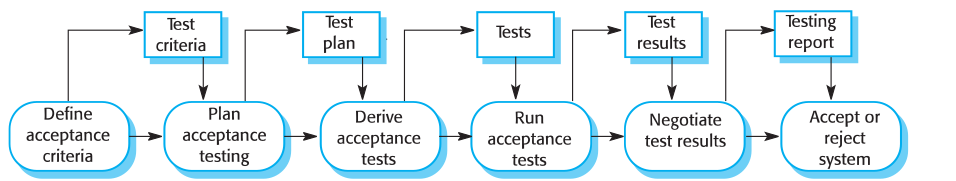
\includegraphics[width=0.7\textwidth]{acceptance_testing_process.png}}
            \end{figure}
        \end{itemize}
    
    
    \item \textbf{test-driven development} is an approach to program development in which you interleave testing and code development. You developed the code incrementally, along with a set of tests for that increment. You don't start working on the next increment until the code that you have developed passes all of its tests.
    \begin{figure}[!htb]
      \makebox[\textwidth][c]{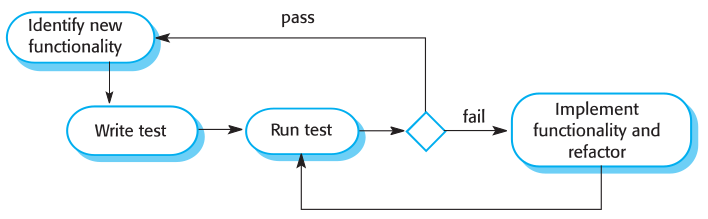
\includegraphics[width=0.7\textwidth]{tdd.png}}
    \end{figure}
    
    \item TDD helps developers clarify their ideas of what a code segment is actually supposed to do: to write a test you need to understand what is intended, as this understanding makes it easier to write the required code. Of course, if you have incomplete knowledge or understanding, TDD won't help.
    
    \item TDD benefits are: \textit{code coverage}, \textit{regression testing}, \textit{simplified debugging}, \textit{system documentation}. One of the most important benefits of TDD is that it reduces significantly the cost of regression testing;
    
    \item TDD is of most value in new software dvelopment where the functionality is either implemented in new code or by using components from standard libraries. Otherwise you need to write tests for used systems as a whole;
    
    \item using the TDD, you still need a system testing process to validate the whole system, that is to check that it meets the requirements of all of the system stakeholders;
    
    \item \textbf{Load Testing}: LT is a kind of Performance Testing which determines a system's performance under real-life load conditions. This testing helps determine how the application behaves when multiple users access it simultaneously. It is commonly used for the Client/Server, Web-based applications; 
\end{itemize}


% ========================================
% ========================================


\newpage
\section{User Stories}
\begin{itemize}
    \item \textbf{User stories} are one of the primary development artifacts for \textit{Scrum} and \textit{Extreme Programming (XP)}. It is a very high-level definition of a requirement, containing just enough information so that the developers can produce a reasonable estimate of the effort to implement it;
    
    \item US. are small, much smaller than other usage requirements artifacts such use cases or usage scenarios;
    
    \item important considerations:
        \begin{itemize}
            \item \textbf{stakeholders write user stories};
            \item use the simple tools to write them, such as \textbf{index cards};
            \item remember non-functional requirements, since stories can be used to describe a\textbf{ wide variety of requirements type};
            \item indicate the \textbf{estimated size to estimate the effort} to implement the US., by assigning to each cards a score, a relative indication of how long it will take a pair of programmers to implement it;
            \item indicate \textbf{the priority}, which is changed and defined by project stakeholders. Cards, basing on prioritization, can be moved around the stack as appropriate;
            \item optionally include a \textbf{unique identifier};
        \end{itemize}

    \item a US. has this format: \textit{as a [role] I want to [something] so that [benefit]}. This approach helps you to think about who a certain feature is built for and why;
    
    \item stakeholders also have the right to define new requirements, change their minds about existing requirements, reprioritize requirements as they see fit and are also responsible for making decisions and providing information in a timely manner;
    
    \item US. affects the planning process on agile stories in \textbf{scheduling area} (the priority assigned to a story affects when the work will be done to implement that requirement) and in \textbf{extimating area} (developers are responsible for estimating the effort required to implement the things which they work on, including stories);
    
    \item there are three common times when stories will be worked on during an agile project:
        \begin{itemize}
            \item during \textbf{inception} phase: in this stage stakeholders creates a stack of user stories as part of requirements evisioning activities to identify the scope of system;
            \item during \textbf{construction} phase: in this stage enw stories are identified, existing stories are splitted (because too large for example), reprioritized or removed (if they are no longer considered to be in scope). So stories evolve over time just like other types of requirements models;
            \item during \textbf{tansition} phase: sometimes new stories will be identified during the Transition phase, although this isn't very common as the focus of release is on hardening the system and not on new functionality
            \begin{figure}[!htb]
              \makebox[\textwidth][c]{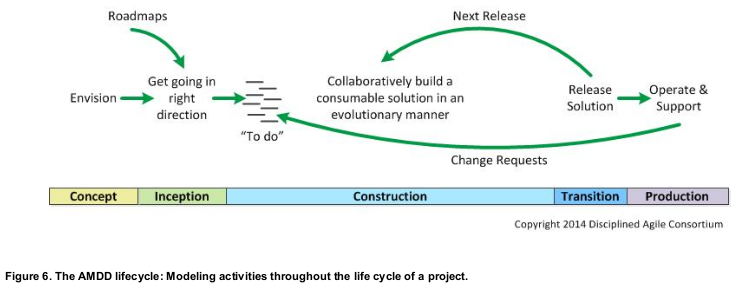
\includegraphics[width=0.85\textwidth]{AMDD_lifecycle.png}}
            \end{figure}
        \end{itemize}
        
    \item because US. contain so little information you will need to flesh them out a bit when you first work with them:
        \begin{itemize}
            \item during \textbf{JIT analysis/model storming with stakeholders}, since is quite common to create screen sketches with stakeholders to exploit what they want;
            \item during \textbf{iteration planning}, since it is common to list programming tasks required to implement the US.;
            \item during \textbf{implementation}, since when you start to work on implementing the user story you may decide to create some rough sketches of what you're going to build, perhaps a flow chart or UML activity diagram representing the relevant business logic;
        \end{itemize}
        
    \item \textbf{epics} are large US., typically ones which are too big to implement in a single iteration and therefore they need to be disaggregated into smaller US. at some point. They are typically lower priority US. because once the epic works its way towards the top of the work item stack, it is reorganized into smaller ones;
    
    \item \textbf{themes} are collections of related US. They are often used to organize stories into releases or to organize them so that various sub-teams can work on them;
\end{itemize}


% ========================================
% ========================================


\section{Splitting the Monolith}
\begin{itemize}
    \item to split the monolith into (micro)services, we need to start from seams. A \textbf{seam} is a portion of the code that can be treated in isolation and worked without impacting the rest of codebase. So we need to identify seams that can become service boundaries.
    \newline
    For example, excellent seams, could be \textit{bounded contexts}. This because, by definition, they represent cohesive and yet loosely coupled boundaries in an organization. \textit{So the first step is to start identifying these boundaries in our code} (a starting point could be \textit{namespaces} concept).
    \newline
    \textbf{First step} so is to create packages (e.g. namespaces) representing these contexts and then move the existing code into them;
    
    \item during this process we can use code to analyze the dependencies between these packages too. Our code should represent our organization, so our packages representing the bounded contexts in our organization should interact in the same way the real-life organizational groups in our domain interact;
    
    \item this process could take an afternoon on a small codebase, or several weeks or months when you're dealing with milions of line of code. It's important that there is no need for this to be a big-bang approach: it is something that can be done bit by bit: an incremental approach will help you learn about the microservices as you go, and will also limit the impact of getting something wrong;
    
    \item now it's time to split the monolith and it is best to think about where we are going to get the most benefit from some part of the codebase being separated, rather than just splitting things for the sake of it. We can start considering:
        \begin{itemize}
            \item the \textbf{pace of changes};
            \item the \textbf{team structure};
            \item a \textbf{security audit}, so that we can provide additional protection to this individual service;
            \item the \textbf{technology} used in a specific package or feature (in term of programming language for example);
            \item \textbf{tangled dependencies}, so we can pull out the seam that is least dependent on. This show, with graphic modelling tools, the seams that are likely going to be harder to disentagle;
            \item the \textbf{database}, by finding seams in our db to so we can split them out cleanly;
        \end{itemize}
    
    \item the first step to split the DB, is to look at the code itself and see which parts of it read to and write from the DB. A common practice is to have a repository layer (for example a framework like Hybernate) to bind the code to the DB, making it easy to map objects or data structure to and from the DB. In this way the code is grouped into packages representing bundled contexts. Having the DB mapping code colocated inside the code for a given context, can help us to understand what part of the DB are used by what bits of code;
    
    \item if there are DB-level constraints (e.g. see paper), which may be a stumbling block, we need to use a tool like \textit{SchemaSpy}, which can generate graphical representations of the relationships between tables. Problems (and solutions) related to that prolem could be:
        \begin{itemize}
            \item if we face with a \textbf{foreign key relationships} problem in which a service \textit{B} wants to access with a foreign key reference to a DB \textit{x} managed by another service \textit{A}, we need to stop the service \textit{B} to reach \textit{X}. Since we don't want the databases integration, the quickest way to address this is to expose the data via an API call in the service \textit{A} that the service \textit{B} can call. However, performing this solution, we loose foreign key relationship and these becomes a constraints that we need to manage in our resulting service rather than in the database level. This may mean that we need to implement our own consistency check across services, or else trigger actions to clean up related data;
            \item if we face with a \textbf{shared static data} problem (e.g. a country code table), options to solve a problem are three: we can duplicate the table for each package (this lead to the potentially consistency challenge), we can deploy these information in a property configuration file of each service (the consistency problem remains even if is more easier to manage), and to push static data to a forth different service (maybe this solution overkill the problem since we are talking about country codes);
            \item if we face with a \textbf{shared mutable data} problem in which a service \textit{A} and a service \textit{B} requires access to a table \textit{X} which can be seen as a domain concept that isn't modelled in the code and is implicitly modelled in the DB. The solution is to create an external service which expose an API to other packages;
            \item if we face with a \textbf{shared table} problem in which, when all the code is merged together, there is a single table to store data relaed to separated concepts that could be stored separately. The solution here is simply to split the table in two;
        \end{itemize}

    \item during database refactoring process, rather than do a big-bang release, it is better to proceed in three phases: firstly split out the schema but keep the service together, the split packages of the monolithic application and finally split monolithic application into services. In this way we give ourselves the ability to revert our changes or continue to tweak things without impacting any consumers of our service;
    
    \item by splitting services, and related databases, we loose the safety afforded to us by having a single transaction: if we have two tables to update together, what happens when the insertion into the first table works but the insertion in the second table fails?
        \begin{itemize}
            \item we may \textbf{try again later} assuming that a retry would fix it. It is also called \textbf{eventual consistency}, in which we can accept that the system will get itself into a consistent state at some point in the future;
            \item we may \textbf{reject the entire operation} putting the system back into a consistent state. What we have to do is a \textbf{compensating transaction}, kicking off a new transaction to wind back what just happened (via a \textit{DELETE} operation for example). Notice that also the compensating transaction could fail, so we need to retry that transaction or to have a some backend process to clean up the inconsistency later on;
            \item we can manually orchestrate compensating transaction by using \textbf{distributed transactions}: they try to span multiple transactions within them, using some overall governing process (\textit{transaction manager}) to orchestrate the various transactions being done by underlying systems. The common algorithm to perform DT is to use a \textbf{two phase commit}: during the first phase (\textit{voting phase}) each participant (called \textit{cohort}) in the DT tells the transaction manager whether it thinks its local transaction can go ahead. If the transaction manager gets a \textit{yes} vote from all cohorts, then it tells them all to go ahead and perform their commits. Using this process we are vulnerable to outages since all problems, related to communication or services alive (?), can block the algorithm or lock resources or etc.;
        \end{itemize}
    To solve this problem see the paper at page 93;
    
    \item the problem of the \textit{reporting process} (operation with which databases are inspected to generate meaningful outputs and reports) is due to presence of all data in the same place (for monolithic applications) and is due to storing data in multiple different systems (for splitted applications). It can be solved in these ways;
        \begin{itemize}
            \item the required data can be \textbf{pulled from the source system} via API calls, so to report across data from two or more systems, you need to make multiple calls to assemble this data. This approach brakes down rapidly with use cases that require larger volume if data.
            \newline
            Reporting systems also often rely on third-party tools that expect to retrieve data in a certain way, and here providing a SQL interface is the fastest way to ensure your reporting tool chain is as easy to integrate with as possible. One of the key challenge is that the API is exposed by the various microservcies may well not be designed for reporting use cases, so this could be inefficient and could generate load for the service in question too.
            \newline
            The nature of reporting is often that we access the long tail of data: this means that we may well request resources that no one else has requested before resulting in a potentially expensive cache miss. A solution to that is to expose batch API to make reporting easier, or to model the batch request as a resource in its own right (e.g. a different endpoint exposed by service). This would allow potentially large datafiles to be exported without the overhead of being sent over HTTP. Moreover the system could simply save a CSV file to a shared location;
            \item rather than have the reporting system pull the data, we could instead have the \textbf{data pushed to the reporting system}: in this way you can have a standalone program that directly access the database of the service that is the source of data, and pumps it into a reporting database. This approach, if implemented properly, shows that the downsidesof the coupling are more than mitigated by making the reporting easier. Moreover the data pump should be built and managed by the same team that manages the service;
            \item if we use a system that can emits events, we can subscribe to the event that notify the state change with an \textbf{event subscriber that pumps data} into the reporting database. The coupling on the underlying database of the source microservice is now avoided. The main downsides to this approach are that all the required information must be broadcast as event, and may not scale as well as data pump for larger volumes of data that has the benefit of operating directly at the database level;
            \item \textbf{backup data pump by netflix} ??
            \newline
            \newline
            \newline
        \end{itemize}
        
    \item we have to consider that any changes of the system becomes to bugs and mistakes, so it is necessary to \textit{understand how best mitigate the cost of those mistakes}. An approach is to try to make mistakes where the impact will be lowest. Another great technique is to adapt an approach used in OO systems; the \textbf{class-responsibility-collaboration (CRC) cards}. With CRC cards you write on one index card the name of the class, its responsibilities and who it collaborates with. When working through a proposed design, for each service are listed its responsibilities in terms of the capabilities it provides, with the collaborators specified in the diagram. As you work through more use cases, you start to get a sense as to whether all of this hangs together properly;
        
    \item \textbf{SAGA pattern}: it is a patterns for distributed transactions. A saga is a sequence of local transactions where each transaction updates data within a single service. The first transaction is initiated by an external request corresponding to the system operation, and then each subsequent step is triggered by the completion of the previous one;
\end{itemize}


% ========================================
% ========================================


\newpage
\section{Cloud Computing}
\begin{itemize}
    \item \textbf{Cloud Computing} is a technological advancement that focuses on the way we design computing systems, develop applications and leverage existing services for building software. It is based on the concept of \textit{dynamic provisioning}, which is applied to services, compute capability, storage, networking and IT infrastructure in general;
    
    \item \textbf{CC} allows renting infrastructures, runtime environments and services on a \textit{pay-per-use basis} and can be classified as new paradigm for the dynamic provisioning of computing services supported by the state-of-the-art data centers employing virtualization technologies for consolidation and effective utilization of resources;
    
    \item in such a model, users access services based on their requirements, without regard to where the services are hosted. By this point of view, cloud computing turns IT services into \textit{utilities};
    
    \item \textit{service orientation} allows cloud computing to deliver its capabilities with familiar abstractions, and \textit{virtualization} confers on cloud computing the necessary degree of customization, control and flexibility for building production and enterprise systems;
    
    \item the \textbf{long-term vision} of cloud computing is that IT services are traded as \textit{utilities} in an open market, without technological and legal barriers. In this \textit{global cloud marketplace}, cloud services providers and consumers, trading cloud services as utilities, play a central role;
    
    \item the Internet plays a fundamental role in cloud computing, since it represents either the \textit{medium} or the \textit{platform} trough which many cloud computing services are delivered and made accessible: \textit{C.C. refers both the applications delivered as services over the internet and the hardware and system software in the datacenters that provide those services};

    \item alongside service orientation view, C.C. introduces concept of \textbf{everything as a service (XaaS)}, where the different components of a system can be delivered, measured and consequently priced as a service;
    
    \item those services are delivered (referring to \textit{utility-oriented approach}) with a given pricing model, and in most cases a \textbf{pay-per-use} strategy. It makes it possible to access online storage, rent virtual hardware or use development platforms and \textit{pay only for their effective usage};
    
    \item The three major models for deploying and accessing cloud computing environments are:
    \begin{itemize}
        \item \textbf{public clouds} are the most common deployment models in which necessary IT infrastructure is established by a third-party service provider that makes it available to any consumer on a subscription basic;
        
        \item \textbf{private clouds} are used by large organizations that own massive computing infrastructure can still benefit from cloud computing by replicating the cloud IT service delivery model in-house. The use of cloud-based in-house solutions is also driven by the need to keep confidential information within an organization's premises;
        
        \item \textbf{hybrid clouds} are used when private cloud resources are unable to meet users' QoS requirements. It is partially composed of public cloud resources and privately own infrastructures;
    \end{itemize}
    
    \item a fundamental characteristic of cloud computing is the capability to deliver, on demand, a variety of IT services that are quite diverse from each other, which creates different perceptions of what C.C. is among users. The categories are:
    \begin{itemize}
        \item \textbf{Infrastructure as a Service (IaaS)}: these type of solutions deliver infrastructure on demand in the form of virtual hardware, storage and networking. Virtual hardware is utilized to provide compute on demand in the form of virtual machine instances. Virtual storage is delivered in the form of raw disk space or object store. Virtual networking identifies the collection of services that manage the networking among virtual instances and their connectivity to the internet or private networks;
        
        \item \textbf{Platform as a Service (PaaS)}: these type of solutions deliver scalable and elastic runtime environments on demand and host the execution of applications. These services are backed by a core middleware platform that is responsible for creating the abstract environment where applications are deployed and executed;
        
        \item \textbf{Software as a Service (SaaS)}: these type of solutions provide applications and services on demand. Most of the common functionalities of desktop applications, such as office automation, document management or photo editing, are replicated on the provider's infrastructure and made more scalable and accessible through a browser on demand;
    \end{itemize}
    
    \item the most \textbf {characteristics and benefits} of C.C. are: no up-front commitments, on-demand access, nice pricing, simplified application acceleration and scalability, efficient resource allocation, energy efficiency and seamless creation and use of third-party services. Moreover the most evident benefit is the increased economical return due to reduced maintenance cost. \textit{For more information look at paper par. 1.1.5};
    
    \item alongside benefits, there are some \textbf{open challenges}: the \textit{dynamic provisioning of cloud computing services and resources} in terms of modality and amount of time, the \textit{service availability}, the \textit{security challenge} in terms of confidentiality, secrecy and protection of data in a cloud environment, and, finally, the \textit{legal issues and privacy in different countries challenge}. \textit{For more information look at paper par. 1.1.6};
    
    \item \textbf{[mainframes, clusters and grids]}..? C. C. is often considered the successor of grid computing. In reality, it embodies aspects of all these three major technologies: are deployed in large datacenters hosted by a single organization, are characterized by the fact of having virtual infinite capacity being fault tolerant as in case of mainframes, in many cases computing nodes of computing clouds are commodity machines, as in the case of clusters and services are available on a pay-per-use basis as introduced in grid computing;
    
    \item \textbf{virtualization} is another core technology for C.C.: it encompasses a collection of solutions allowing the abstraction of some of the fundamental elements for computing, such as hardware, runtime environments, storage and networking. It confers that degree of customization and control that makes cloud computing appealing for users and, at the same time, sustainable for cloud services providers;
    
    \item \textbf{it} is essentially a technology that allows creation of different computing environments to simulate the interface that is expected by a guest. The most common example of virtualization is the \textit{hardware virtualization}: this technology allows simulating the hardware interface expected by an operating system (example solutions are Amazon EC2, VMware, vCloud ..).
    
    \item virtualization allows the coexistence of different software stacks on top of the same hardware. These stacks are contained inside \textbf{virtual machines}, which operate in complete isolation from each other. High performance servers can host several virtual machines instances, thus creating the opportunity to have a customized software stack \textit{on demand};
    
    \item virtualization technologies are also used to replicate runtime environments for programs: applications in the case of \textit{process virtual machines} (e.g. Java or .NET) instead of being executed by the operating system, are run by a specific program \textit{virtual machine}. This technique allows isolating the execution of applications and providing a finer control on the resource they access;
    
    \item the core reference model for cloud computing systems is the \textbf{Service-oriented Computing (SOC)} by adopting the concept of services as the main building block of application and system development;: it supports the development of rapid, low-cost, flexible, interoperable and evolvable applications and systems;
    
    \item a \textbf{service} is an abstraction representing a self-describing platform-agnostic component that can perform anyhing from a simple function to a complex business process. It is \textit{loosely coupled}, \textit{reusable}, \textbf{programming language independent} and \textit{location transparent}. They are aggregated into a \textbf{Service Oriented Architecture (SOA)} which is a logical way of organizing software systems to provide end user or other entities distributed over the network  with services through published and discoverable interfaces;
    
    \item the SOC introduced the fundamentalconcept of \textbf{Quality of Service (QoS)}, which identifies a set of functional and non-functional attributes that can be used to evaluate the behavior of a service from different perspective;
    
    \item \textbf{Utility-oriented computing} is a vision of computing that defines a service-provisioning models for compute services in which resources such as storage, compute power, applications and infrastructure are packages and offered on a pay-per-use basis;
    
    \item \textbf{Heroku's Dynos}: the Heroku Platform uses the container model to run and scale all Heroku apps. The containers used at Heroku are called “dynos.” \textbf{Dynos} are isolated, virtualized Linux containers that are designed to execute code based on a user-specified command. Your app can scale to any specified number of dynos based on its resource demands. Heroku’s container management capabilities provide you with an easy way to scale and manage the number, size, and type of dynos your app may need at any given time. Dynos are the building blocks that power any Heroku app, from simple to sophisticated;
    
    \item \textbf{Functions as a Service}; FaaS is a serverless way to execute modular pieces of code on the edge. FaaS lets developers write and update a piece of code on the fly, which can then be executed in response to an event, such as a user clicking on an element in a web application. This makes it easy to scale code and is a cost-efficient way to implement microservices;
    
    \item \textbf{Lock-in problem}: it makes a customer dependent on a vendor for products or services, unable to use another vendor without substantial switching costs. The higher the cloud layer you operate in, the greater the lock-in. It can be avoided/reduced following these tips:
        \begin{itemize}
            \item carefully choose provider;
            \item date providers don’t marry them;
            \item think carefully before using proprietary cloud-vendor services;
            \item reconsider the way you think about purchasing services;
            \item plan your exit strategy;
            \item ensure portability of data;
            \item use unified interfaces;
            \item choose open standards and open-source technologies;
            \item use multiple clouds;
            \item use loosely coupled architecture, API/REST integration;
            \item use microservices architectures;
            \item use containers and devops tools;
        \end{itemize}
\end{itemize}


% ========================================
% ========================================


\section{Docker}
\begin{itemize}
    \item \textbf{Docker} is a Linux-based platform for developing, shipping and running applications through container-based virtualization. \textbf{Container-based virtualization} exploits the kernel of host's operating system to run multiple isolated user-space instances, called \textbf{containers};
    
    \item docker platform is good for:
        \begin{itemize}
            \item \textit{replace virtual machines} if the user only care about the application and not the operating system;
            \item \textit{prototyping software} if the user want to quickly experiment with software without either disrupting existing setup or going through the assale of provisioning a VM;
            \item \textit{packing software} since a docker image has no dependencies for a Linux user and he can build his image and can be sure that it can run on any modern Linux machine;
            \item \textit{enabling a microservices architecture} since it facilitates the decomposition of a complex system to a series of composable parts;
            \item \textit{modelling networks} because the user can spin up hundreds of isolated containers on one machine, and modelling a network is a breeze;
            \item \textit{enabling a full-stack productvity when offline} by bundle all the parts of the system into Docker containers;
            \item \textit{reducing debugging overhead}, since with Docker we can reproduce and debug the bug and the environment much simply;
            \item \textit{documenting software dependencies and touchpoints} since Docker force to document explicitly the software dependencies;
            \item \textit{enabling continuous delivery paradigm} since Docker builds are more reproducible and replicable than trafitional software building methods. Moreover it make more simpler the \textbf{Blue/Green} (where "live" and "last" deployments are maintained on live) and \textbf{Phoeix Deployment} (where whole systems are rebuilt on each release) techniques;
        \end{itemize}
        
    \item key concepts of docker are:
        \begin{itemize}
            \item \textbf{images}: collection of filesystems layers and some metadata (e.g. environment variables, port mapping, volumes). They can be seen as read-only templates that includes exactly what they need to run applications and providing all instructions needed for creating and configuring a container;
            \item \textbf{containers} a running instance of an image. They can be seen as packages containing software dependencies which isolate the application from the guest system, share kernel of the operating system. They can be seen as the standard unit inside of which the applications are executed. Inside them, changes to a file are stored withing a container in acopy-on-write mechanism. They are created from images, inherit their filesystems, and use their metadata to determine their startup configurations. The base image cannot be affected by a container;
            \item \textbf{layers}: a collection of changes to files;
        \end{itemize}
    \item \textbf{docker layering} helps to manage the big problem of increasing size of containers when new istances are created. By default, Docker internally uses a \textit{copy-on-write} mechanism to reduce the amount of disk space required. Whenever a running container needs to write a file, it records the change by copying that file to a new area of disk, When a Docker commit is performed, this new area of disk is frozen and recorded as a layer with its own identifier;
    
    \item more specifically, \textbf{copy-on-write} is a standard optimization strategy used in computing: when user creates a new object from a template, data are copied only when it's changed, rather than copying the entire set of required data immediately;
    
    \item to preserve data on stopping containers, Docker \textbf{volumes} are introduced, which are especially-designated directories whose purpose is to persist data, independently of the container's lifecycle mounting them;
    
    \item containers can communicate with each other by creating virtual networks (from simple bridge to complex overlay);
    
    \item existing docker images are distribute through so-called Docker \textbf{registries} and new images can be built by extending ones;
    
    \item a \textbf{dockerfile} is a special file which allows us to create a docker image executing precise commands;
    
    \item \textbf{benefits} are: a simplified deployment, rapid availability, a more granular control, simplified testing operations;
\end{itemize}


% ========================================
% ========================================


\newpage
\section{Fog Computing}
\begin{figure}[!htb]
    \makebox[\textwidth][c]{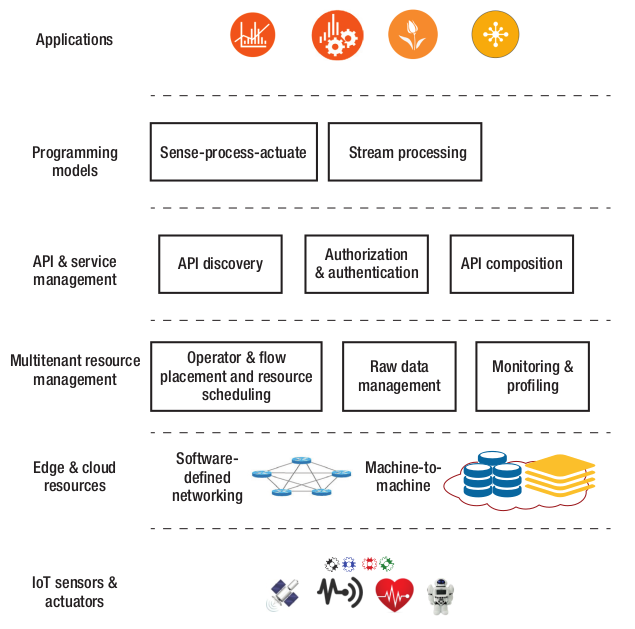
\includegraphics[width=0.37\textwidth]{fog_computing_architecture.png}}
\end{figure}
\begin{itemize}
    \item \textbf{Fog computing} is a distributed paradigm that provides cloud-like services to network edge. It was born to address problems linked to big amount of data coming from IoT devices by leveraging cloud resources and coordinating the use of geographically distributed edge devices. It seamlessly integrates edge devices and cloud resources, to avoids resource contetion at the edge by leveraging cloud resources and coordinating the use of geographicaly distributed edge devces;
    
    \item this technology deals with IoT data locally by utilizing clients or edge devices near users to carry out a substantial amount of storage, communication, control, configuration and management;
    
    \item fog systems generally use the \textbf{sense-process-actuate} and \textbf{stream-processing} programming models: sensors stream data to IoT networks, applications running on fog devices subscribe to and process the information and the obtained insights are translated into actions and sent to actuators. Moreover Fog systems can dynamically discover and use APIs to build complex functionalities;
    
    \item edge and cloud resources communicate using M2M standards as MQTT and COAP;
    
    \item the most prominent software systems for building fog computing environments and applciations are:
    \begin{itemize}
        \item \textbf{Cisco IOx} provides device management and enables M2M services in fog environments;
        \item \textbf{Cisco Data in Motion (DMo)} enables data management and analysis at the network edge;
        \item \textbf{LocalGrid}'s fog computing platform is a software installed on the network devices in smart grids;
        \item \textbf{Cisco PartStream}'s fog computing platform enables real-time IoT analytics;
    \end{itemize}
    
    \item Fog computing applications:
    \begin{itemize}
        \item fog computing could be useful in \textbf{helathcare}, in which real-time processing and event response are critical. One proposed system utilizes fog computing to detect, predict and prevent falls by stroke patients. A propsed fog computing-based smart-healtcare system enables low latency, mobility support and location and privacy awareness;
        \item fog computing can be used with \textbf{smart utility services}, whose focus is improving energy generation, delivery and billing. In such environments, edge devices can report more fine-grained energy-consumption details to users' mobile devices than traditional smart utility services;
        \item fog computing plays a major role in \textbf{augmented reality applications} which are latency sensitive. For example EEG Tractor Beam augmented multiplayer, online brain-computer-interaction game performs continuously real-time brain-state classification on fog devices and then tunes classification models on cloud servers. Also wearable cognitive-assistance system that uses Google Glass devices helps people with reduced mental acuity perform various tasks: in these application evices communicate with the cloud for delay-tolerant jobs such as errors reporting and logging;
    \end{itemize}
    
    \item to test fog computing implementations the open source simulator \textbf{FogSim} is developed: it enables the modelling and simulation of the evaluation of resource-management and scheduling policies across the edge and cloud resources under multiple scenarios, based on their impact on latency, energy consumption, network congestion and operational costs;
    
    \item realizing fog computing's full potential presents several challenges including balancing load distribution between edge and cloud resources. Others \textbf{fog challenges} are:
    \begin{itemize}
        \item enable \textbf{real-time analytics} to dynamically determine which analytics tasks are being published to which cloud or edge-based resource to minimize latency and maximize throughput;
        \item \textbf{add and remove resources dynamically} because processing nodes are generally mobile devices that frequently join and leave networks;
        \item \textbf{designing and implementing} authentication and authorization techniques that can work with multiple fog nodes that have different computing capacities is difficult. PKI and trusted execution environments are potential solutions. Moreover, to help users of fog deployment to plan for the failure of fog elements, they could apply standards, such as the \textit{Stream Control Transmission Protocol}, that deal with packet and event reliability in wireless sensors network;
        \item because the computation is distributed, in could be less energy efficient than centralized cloud systems. Using efficient communication protocols (e.g. \textit{COAP}), effective filtering and sampling techniques, network resource optimization can minimize \textbf{energy consumption} in fog environments;
    \end{itemize}
\end{itemize}


% ========================================
% ========================================


% ========================================
% ========================================


\section{FogTorch$\Pi$ - Modelling costs}
\begin{itemize}
    \item modern applications usually consists of many independent deployable components. When deciding to deploy that application components, one should check their hardware, software, IoT, and QoS requirements against the offerings of the available context infrastructure. \textit{Determining eligible deployments of a multi-component application to a given Fog infrastructure is an NP-hard problem};
    
    \item estimating deployment costs is very important to industry and business which aim at minimising deployment operational costs at runtime, having both to fulfil user requirements and to maximize their revenues;
    
    \item tools to support app deployment to the Fog should desirably feature \textit{QoS-awareness} (to latency reduction, bandwidth saving), \textit{context-awareness} (to suitably exploit local ad remote resources) and \textit{cost-awareness} (to enact cost-effective deployments);
    
    \item \textbf{FogTorch$\Pi$} II is a prototype that determine app deployments that meet alll processing, IoT and QoS requirements over a given infrastructure, estimates their QoS-assurance and Fog resource consumption by simulating latency and bandwidth variations of communication links as per given probability distribution. The new version of FogTorch$\Pi$ can help IT experts in deciding how to distribute application components to Fog infrastructures in a QoS-, context- and cost-aware manner;
    
    \item \textit{see on papere for 'motivating example'}
    \begin{figure}[!htb]
        \makebox[\textwidth][c]{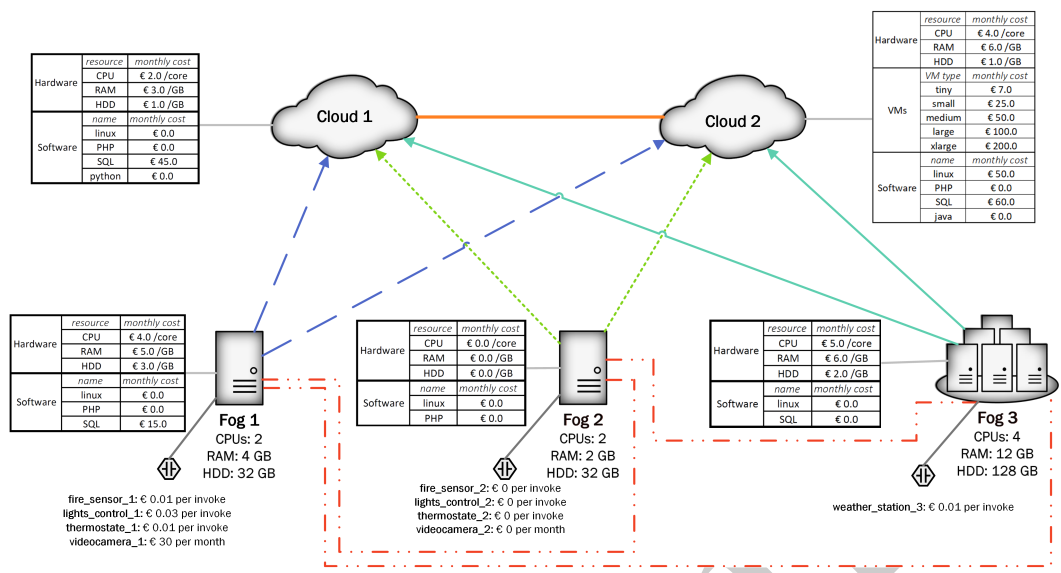
\includegraphics[width=0.8\textwidth]{fog_infrastructure.png}}
    \end{figure}
    
    \item the first version of FogTorch$\Pi$ takes as input:
        \begin{itemize}
            \item an \textit{IoT+Fog+Cloud infrastructure}, as shown in previous figure, with the specification (including also HW, SW and IoT capabilities) of Fog and Cloud nodes available for deployment and the probability distribution of measures featured by the communication links interconnecting such nodes;
            \item a \textit{multi-component application A}, specifying HW, SW and IoT requirements of each components and QoS needed to support component-component and component-Thing interactions;
            \item a \textit{Things binding $\vartheta$}, mapping each IoT requirement of an application component to an actual Thing I;
            \item a \textit{deployment policy $\delta(\gamma$)}, white-listing the nodes where component $\gamma$of A can be deployed according to security or business-related constraints;
        \end{itemize}
        
    \item based on such input, FogTorch$\Pi$ determines all the eligible deployments of the components of A to Cloud or Fog nodes I. An \textit{eligible deployment $\Delta$} maps each component $\gamma$ of A to Cloud or Fog node \textit{n} in \textit{I} so that
    \begin{itemize}
        \item $n \in \delta(\gamma)$ and it satisfies the processing requirements of $\gamma$;
        \item hardware resources are enough to deploy \textit{all} the components of \textit{A} mapped to \textit{n};
        \item Things specified in $\delta$ are reachable;
        \item component-component and component-Thing interaction link do not exceed the available bandwidth and meet their latency requirements;
    \end{itemize}
    
    \item FogTorch employs the Monte Carlo method to estimate the \textit{QoS-assurance} of output deployments, by aggregating the eligible deployments obtained when varying the QoS of communication links (as per their input probability distribution). In addition, FogTorch outputs the percentage of resources (RAM and HDD) consumed in the Fog layer (or specified Fog nodes) after performing an eligible deployment;
    \begin{verbatim}
procedure MONTE CARLO (A, I, θ, δ, n)
	D = 0               // dictionary of <<delta>, counter>
	for n times do
		I_s = SAMPLELINKSQoS (I)
		E   = FINDDEPLOYMENTS (A, I_s, θ, δ)
		D   = UNIONUPDATE (D, E)
	end for

	for <delta> in keys(D) do
		D[<delta>] = D[<delta>]/n
	end for
	
	return D
end procedure
    \end{verbatim}
    
    \item at the end of simulation (for \textit{n$\geq$100000}, the QoS-assurance is the percentage of runs a certain deployment $\Delta$ was found in $FNDDEPLOYMENTS (A, I_s, \theta, \delta)$. Such percentage estimates how likely $\Delta$ is to meet all QoS constraints of A, taking into account variations in the communication links as per historical behavior of \textit{I};
    
    \item for the \textbf{cost model} of FogTorch$\Pi$ see paper!
\end{itemize}

\newpage


\section{SecFog}
\begin{itemize}
    \item regarding the \textit{security}, Fog computing on one hand will increase the number of security enforcement points by allowing local processing of private data closer to the IoT sources and, on the other hand, it will be exposed to brand new threats of what concerns the trust and the physical vulnerabilities of devices. So there is a clear need to evaluate a priori whether an application will have its security requirements fullfilled by the nodes chosen for the deployment of it components. Furthermore it is important that the techniques employed to reason on security properties of deployed multi-component applications are configurable and well-founded;
    
    \item in the figure below are listed security features that can be offered by Cloud and Fog nodes. Features that are common with the cloud might assume renewed importance in Fog scenarios, due to the limited capabilities of the available devices;
    \begin{figure}[!htb]
      \makebox[\textwidth][c]{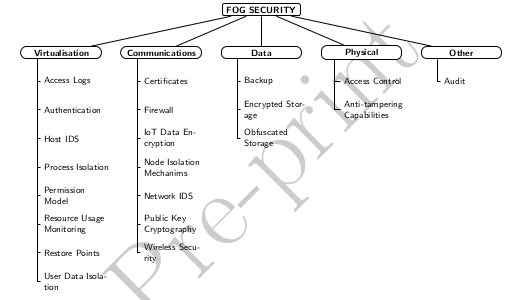
\includegraphics[width=0.5\textwidth]{taxonomy.png}}
    \end{figure}
    
    \item in the figure below is exposed a general view of Secfog: for each managed node, the operator publishes a \textbf{Node Descriptor (ND)} featuring a list of the node security capabilities along with a declared measure of their reliability (in the range [0,1]). On the other hand, based on the same vocabulary, application operators can define \textbf{custom security policies}, which can complete or override \textbf{default security policies} available in SecFog implementation. Custom and default properties are used, along with ground facts, to specify the \textbf{security requirements} of a given application as \textbf{Component Requirements (CR) and Application Requirements (AR)} or both. Finally the security level of an \textit{application deployment} can be assessed by matching the security requirements of the application with the security capabilities featured by the infrastructure  and by multiplying the reliability of all exploited security capabilities, weighting them as per \textit{trust degree}, which may be assigned by application deployers to each infrastructure operator;
    \begin{figure}[!htb]
      \makebox[\textwidth][c]{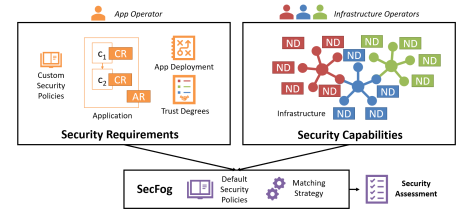
\includegraphics[width=0.5\textwidth]{sec_fog_general.png}}
    \end{figure}
    
    \item \textbf{example}
    \begin{figure}[!htb]
      \makebox[\textwidth][c]{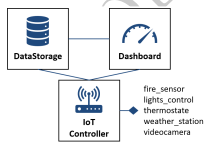
\includegraphics[width=0.4\textwidth]{fog_example.png}}
    \end{figure}
    
    \item to implement SecFog model and the matching strategy, the language \textit{ProbLog} is used. It is a Python package that permits writing logic programs that encode complex interactions between large sets of heterogeneous components, capturing the inherent uncertainties that are present in real-life situations;
    
    
\end{itemize}


% ========================================
% ========================================

\end{document}